\paragraph{What is Statistical Learning?}
Notation:
\begin{itemize}
 \item \textbf{Input variables}: predictors, independent variables
   features or variables.
 \item \textbf{Output variables}: response, dependent variables.
\end{itemize}
When we observe a \tB{quantitative response $Y$} knowing there are 
\tB{$p$ predictors} such as\\
$X=\left( X_{i} \right)_{1\leq i\leq p}$ then we write:
\enc{$Y=f\left( X \right)+\epsilon$}\\
$\begin{cases}
f\text{ is some fixed but unknown function of }X\text{ 
and represents the systematics information that }X\text{ provides
about }Y\\
\epsilon\text{ is a random error term, independent of X and has mean }0
\end{cases}
$
\begin{figure}[h]
  \centering
  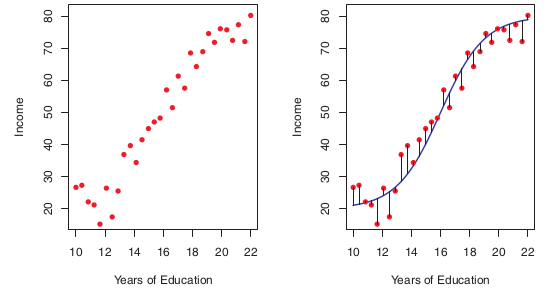
\includegraphics[width=.5\textwidth]{./chap/1chap/1sec/1images/1_1estimationOfF.png}
  \caption{Estimation of $f$}
  \label{fig:1.1}
\end{figure}\\
\begin{figure}[H]
  \centering
  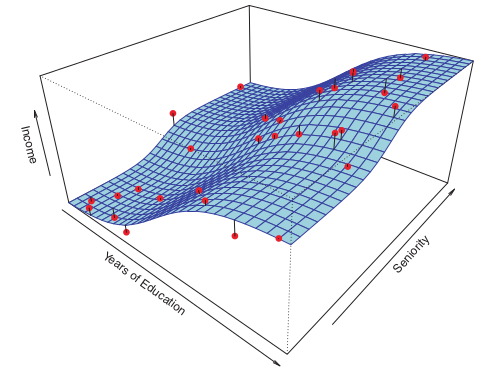
\includegraphics[width=.5\textwidth]{./chap/1chap/1sec/1images/1_2estimationF2D.png}
  \caption{Estimation of $f$ in $2-D$}
  \label{fig:1.1}
\end{figure}
In essence \textbf{Statistical Learning} refers to a set of approaches
for estimating $f$.
\paragraph{Why estimate $f$}
\subparagraph{Prediction}
\encV{$\widehat{Y}=\widehat{f}\left( X \right)$}
$
\begin{cases}
  \widehat{f}\text{ represents our estimating for }f\\
  \widehat{Y}\text{ represents the resulting prediction for }Y
\end{cases}$\\
$\widehat{f}$ is often treated as a \emph{black box} since \tB{we pay
more attention to its prediction accuracy than its exact form}.\\
The accuracy of $\widehat{Y}$ depends on $2$ quantities\\
$\begin{cases} 
  reductible~error\text{, can be \tB{improved by using most appropriate
  statistical learning technique}}\\
  irreductible~error\text{, cannot be changed and \tB{have external 
  causes which are out of control}}
\end{cases}$\\
 simple calculus shows that:
\begin{align*}
  \E{\left[Y-\widehat{Y}\right]^{2}}&=\E{\left[f\left( X \right)+\epsilon-\widehat{f}\left( X \right)\right]^{2}}\\
  &= \underbrace{\E{\left[ f\left( X \right)-\widehat{f}\left( X \right) \right]^{2}}}_{Reducible}+\underbrace{\V{\epsilon}}_{Irreducible}\text{ think that $\E{\epsilon}=0$}
\end{align*}
\subparagraph{Inference} Now we want to know how $Y$ evolves when $X$
changes, so we cannot considerate anymore $f$ as a black box.\\
\begin{itemize}
\item \emph{Which predictors are associated with the response?} (\tB{to
discover variables which have the most important influence therewith 
to reduce number of considered variables})
\item \emph{What is the relationship between the response and each
  predictor?}(\tB{Which components increase Y value and which decrease
  it})
\item \emph{\tB{Can the relationship between $Y$ and each predictor be
	adequately summarized using linear equation} or is the relationship
more complicated?}
\end{itemize}
\paragraph{How do we estimate $f$}
\subparagraph{Aim} Let $(i,j)\in\inter{1}{n}\times\inter{1}{p}$ and 
\tB{$x_{ij}$ represent the value of the $j^{th}$ predictor for $i^{th}$
observation}. Correspondingly let $y_{i}$ represent the response 
variable for the $i^{th}$ observation.\\
Then our training data consists of $\left\{ \left( x_{i},y_{i}
\right)_{1\leq i\leq n}\right\}\text{ where }x_{i}=\begin{pmatrix}
x_{i1}\\.\\.\\.\\x_{ip}\end{pmatrix}$.\\
\tR{We want to find a function $\widehat{f}$ such that $Y\approx
\widehat{f}\left( X \right)$ for any observation $\left( X,Y \right)$}
\subparagraph{Parametric methods}
\begin{enumerate}
	\item \tB{\emph{Assumption about functional form of $f$}}\\ For
		example: $f\left( X \right)=\beta_{0}+\su{{i=1}}{p}
		\beta_{i}X_{i}$ in this case instead to estimate 
		entirely $p$-dimensional function $f$ we only need to
		estimate $\left( \beta_{i} \right)_{0\leq i\leq p}$
  \item After the model selection, \tB{we need a procedure which uses
\emph{data training} to \textit{fit} or \textit{train} the model}.
    \\For example we need to estimate
    $\left( \beta_{i} \right)_{0\leq i\leq p}$ such that:
    $Y\approx\beta_{0}+\su{{i=1}}{p}\beta_{i}X_{i}$\\ The most common
    approach to fit the model is \emph{least squares}.
\end{enumerate}\encV{
The parametric methods allow to reduce the problem of estimating $f$
down
to one of estimating a set of parameters}.
\begin{figure}[H]
\begin{subfigure}{0.5\textwidth}
  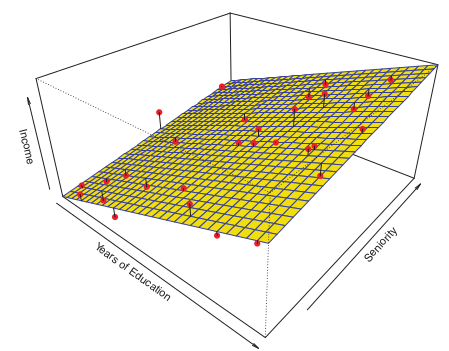
\includegraphics[width=0.9\linewidth, height=5cm]{./chap/1chap/1sec/1images/1_3linearEstimation.png} 
  \caption{Linear estimation:\\$income=\\\beta_{0}+\beta_{1}\times education+\beta_{2}\times seniority$}
  \label{fig:1.3_1}
\end{subfigure}
\begin{subfigure}{0.5\textwidth}
  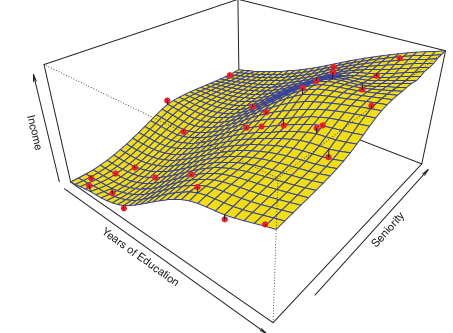
\includegraphics[width=0.9\linewidth, height=5cm]{./chap/1chap/1sec/1images/1_4BestEstimation.png} 
  \caption{Best estimation of $f$ for\\ $income\approx f\left( income,seniority \right)$}
  \label{fig:1.3_2}
\end{subfigure}
\caption{Estimation of $f$ with 2 degrees of precision}
\label{fig:1.4}
\end{figure}

\subparagraph{Non-Parametric methods}
Any parametric approaches brings with it the possibility that the
functional form used to estimate $f$ is very different from the true
$f$. In contrast non-parametric approaches completely avoid this danger
since \tB{no assumption about the form of $f$ is made.} But non
parametric approaches do suffer from non-reducing problem, and \sB{they
need a very greater number of observation than with parametric 
approaches}.
\paragraph{The trade-off between Prediction Accuracy and model
Interpretability}
When inference is the goal, there are clear advantages to using simple
and relatively inflexible statistical learning methods.
\begin{figure}[H]
   \centering
   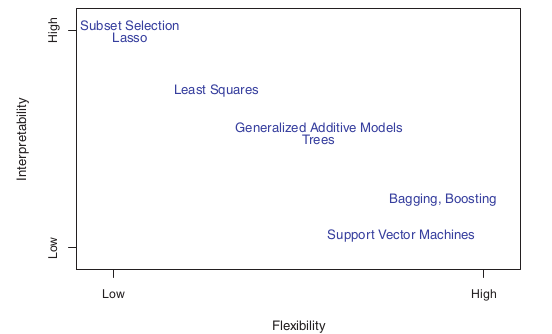
\includegraphics[width=.7\textwidth]{./chap/1chap/1sec/1images/1_5ToChooseAgoodApproach.png}
   \caption{To know which methods to use.}
   \label{fig:1.4}
 \end{figure}
 \paragraph{Supervised versus unsupervised learning}
 We speak about \tR{\emph{supervised problems}} \sR{when for each predictors
 $x_{i}$ there is an associated response measurement $y_{i}$}.\\
 Whereas in \tR{\emph{unsupervised problems}} \sR{we observe a vector of
 measurements $x_{i}$ but not associated response $y_{i}$}. Then we can
 seek to understand the relationship between the variables or between
 observations.\\ One statistical tool that we may use in this setting
 is \emph{clustering}
 \begin{figure}[H]
   \centering
   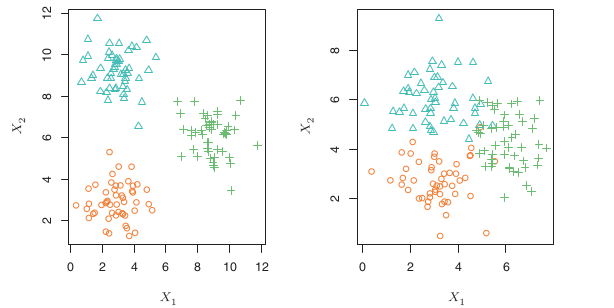
\includegraphics[width=.7\textwidth]{./chap/1chap/1sec/1images/1_6Clustering.png}
   \caption{Clustering methods is used for \emph{unsupervised problems}.}
   \label{fig:1.5}
 \end{figure}
 \paragraph{Regression versus Classification problems}
 In general Regression is used for quantitative variables whereas
 classification is used for qualitative variables but we can find
 several counter-examples.
